% !TEX root = ../main.tex

\documentclass[../main.tex]{subfiles}
\begin{document}

\section{Visualizing trends}
In this next page, we include a \textit{qualitative} chart for visualizing trends in research as we explained them. We want to stress this is not a bibliometric paper, nor is the chart supposed to represent fixed, agreed upon values. Instead, the intended aim is to show how trends in DCS and AI research intertwined and influenced each other throughout the decades, as we did in the History chapter, from a bird's eye view.

The chart is organized as follows: when holding the sheet of paper sideways, the vertical axis represents how symbol oriented every piece of research is. The vertical axis is not a strict symbol-network distinction, but (a) organized as a spectrum, as most research papers are not completely on one side or the other, and (b) representative of the research focus more than the strict content. As an example, let's consider the paradigm of embodied cognition: its interest towards lower level processes and beliefs about their relative complexity does not directly mean they would use Neural Networks to implement decisional processes; in fact, for most robotics-oriented work of the period neural networks would not have been a good choice, due to the limited computing power. Still, the insurgence of such a paradigm shows an interest towards processes that are not limited to high-level rational thoughts or symbolic reasoning, so Brooks' research was not placed strongly in symbolic territory.

The horizontal axis, instead, represents time. Once again, for illustrative purposes, time placements are not exact, as they aren't meant to be. Colors were used to distinguish DCS research, in red, and research that was Computer Science - Mathematics - Artificial Intelligence - Engineering oriented. Lastly, we mention that, of course, only a portion of the works mentioned in the text were represented, itself a portion of published research.

\newpage

\begin{figure}[H]
    \makebox[\linewidth]{
        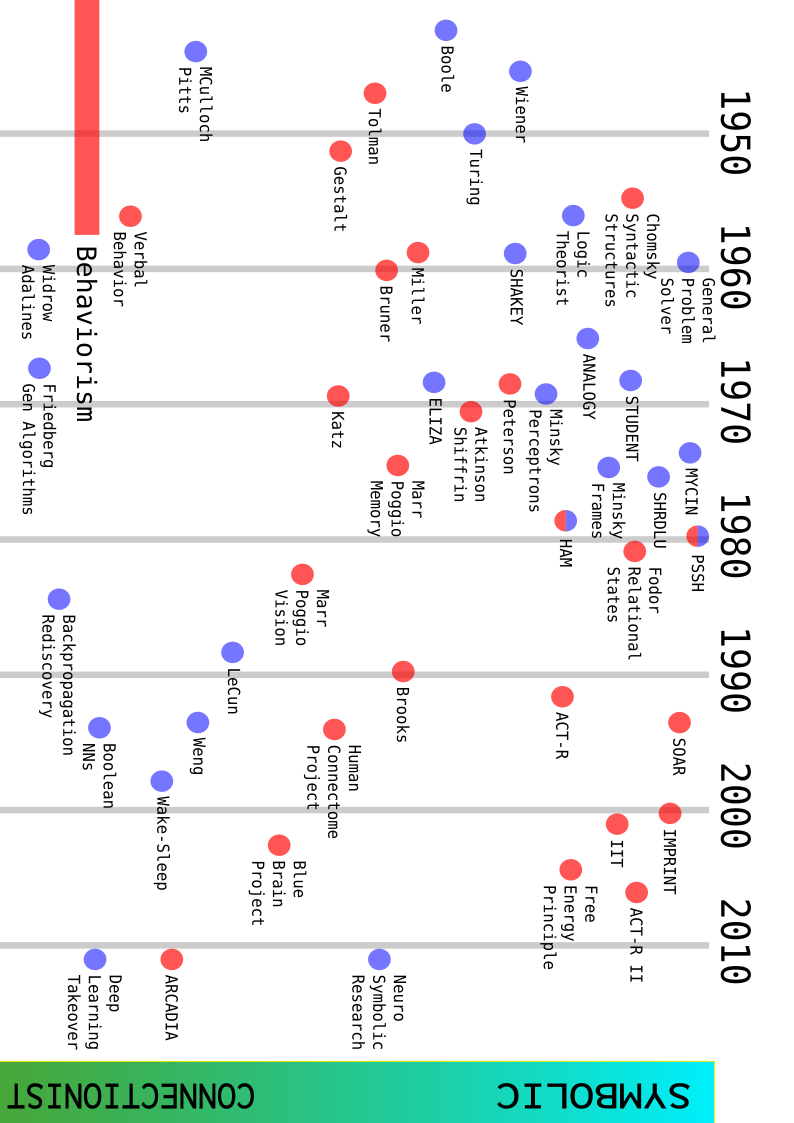
\includegraphics[width=\linewidth]{img/spectrumRotated.png}
    }
    \caption{Research trends, visualized.}
\end{figure}


\end{document}